\esSezione{Moltiplicatore di Booth}\label{sec:esercizio7-1}

\begin{traccia}
Progettare, implementare in VHDL e testare mediante simulazione un moltiplicatore di Booth in grado di calcolare il prodotto di due stringhe da 8 bit, interpretate come numeri con segno in complemento a due.
\end{traccia}

\progetto

L'algoritmo di Booth moltiplica numeri con segno in complemento a due esaminando, a ogni passo, la coppia formata dal bit meno significativo del moltiplicatore e dal bit scartato al passo precedente. Detti \texttt{q0} e \texttt{qm1} tali bit, si hanno tre casi:

\begin{enumerate}
  \item se la coppia vale $00_2$ oppure $11_2$, viene eseguito soltanto lo shift aritmetico a destra;
  \item se vale $01_2$, il moltiplicando viene sommato alla parte alta del prodotto parziale, poi si effettua lo shift;
  \item se vale $10_2$, il moltiplicando viene sottratto alla parte alta, poi si effettua lo shift.
\end{enumerate}

Il calcolo richiede otto passi, uno per bit del moltiplicatore, e il sistema è diviso in parte operativa e unità di controllo. La parte operativa contiene il registro \texttt{M} (moltiplicando), il registro \texttt{A} (parte alta del prodotto parziale), il registro \texttt{Q} (moltiplicatore e parte bassa del prodotto), il flip-flop \texttt{Q[-1]}, un addizionatore/sottrattore a 8 bit e un contatore modulo 8 per contare i passi. L'unità di controllo è una FSM: produce i comandi per i registri e legge \texttt{q0}, \texttt{qm1} e \texttt{last}. Lo schema è visibile in figura~\ref{fig:esercizio7-1:schema}.

\begin{figure}[H]
  \centering
  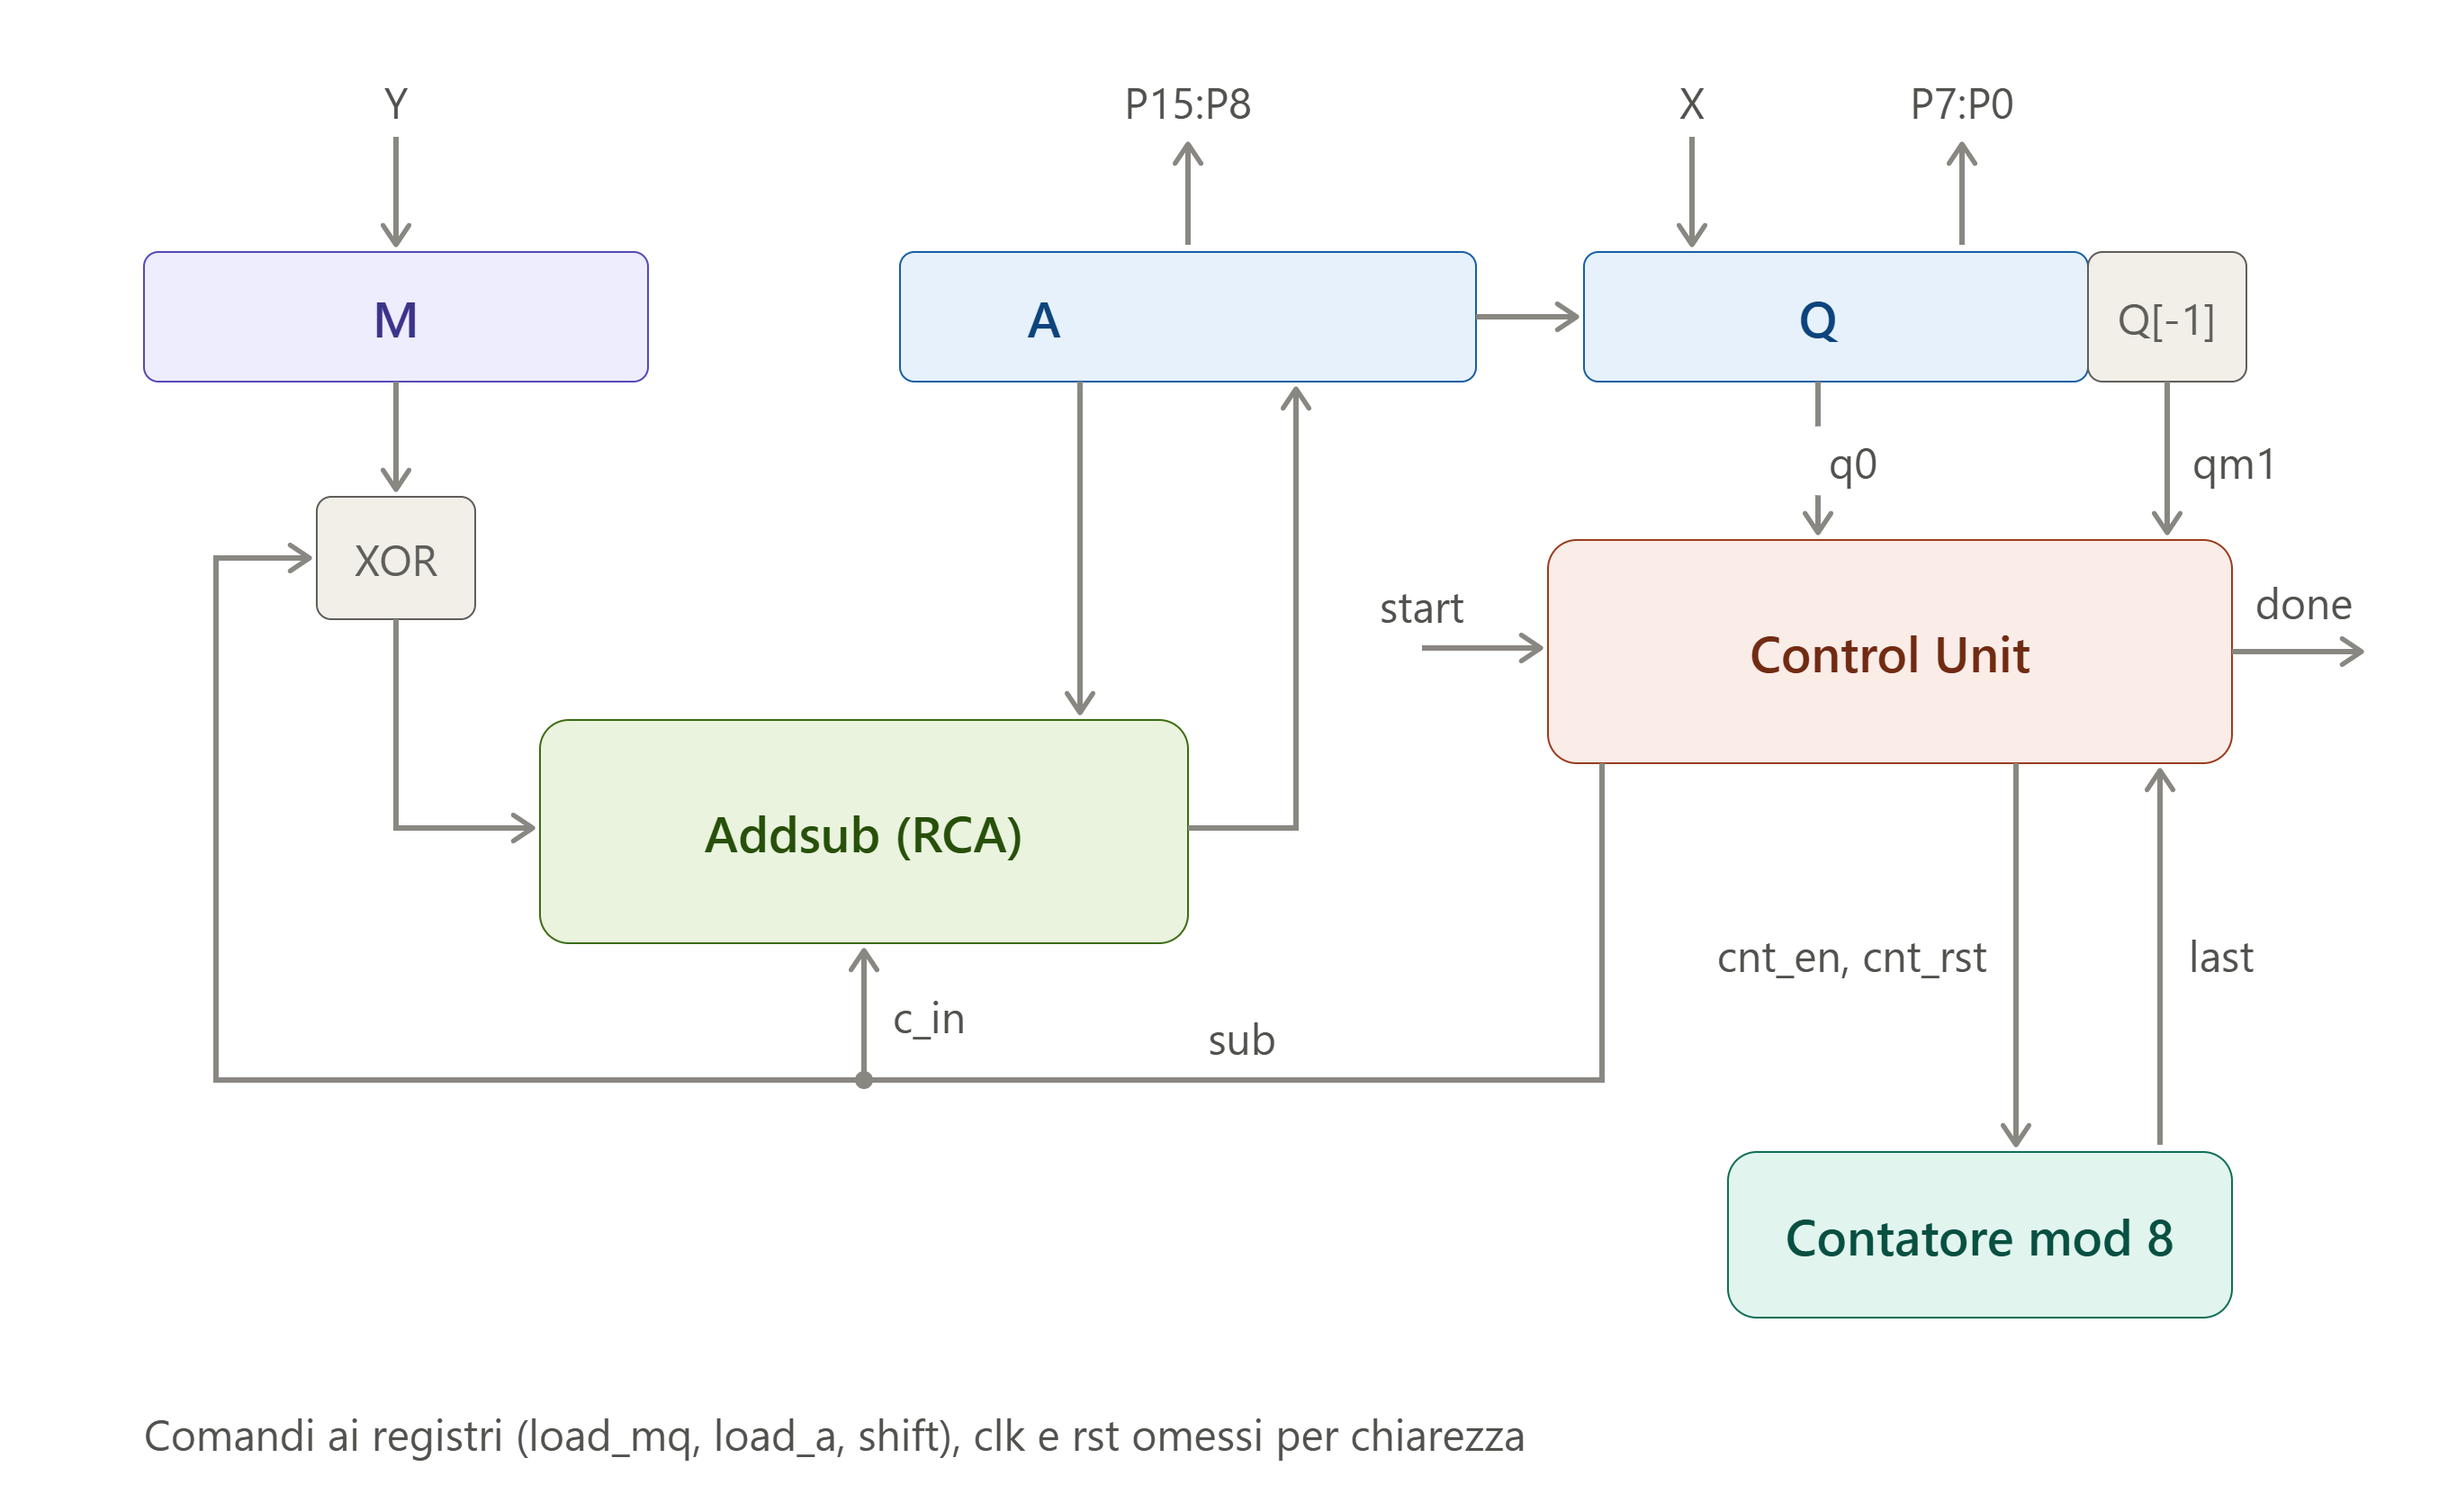
\includegraphics[width=0.7\linewidth]{figure/esercizio7-1/schema}
  \caption{Architettura del moltiplicatore di Booth}
  \label{fig:esercizio7-1:schema}
\end{figure}

Il sommatore riceve \texttt{A} e \texttt{M}, quest'ultimo attraverso uno strato di XOR pilotato da \texttt{sub}. Lo stesso segnale è anche il riporto in ingresso: con \texttt{sub} a \texttt{'1'} si ottiene $A - M$, con \texttt{sub} a \texttt{'0'} si ottiene $A + M$. Il risultato viene ricaricato in \texttt{A}, mentre il prodotto a 16 bit è la concatenazione di \texttt{A} e \texttt{Q}.

A differenza della soluzione proposta nel documento di riferimento, registri e shift register non sono istanziati come componenti separati: \texttt{M}, \texttt{A}, \texttt{Q} e \texttt{Q[-1]} sono segnali aggiornati da un unico process della parte operativa. Il contatore è invece quello parametrico già utilizzato altrove (\texttt{counter\_mod}), non uno dedicato.

\implementazione

Si riportano di seguito i componenti in ordine bottom-up, a partire dal \texttt{full\_adder}: tre ingressi (\texttt{a}, \texttt{b}, \texttt{c\_in}), due uscite (\texttt{s}, \texttt{c\_out}) e architettura dataflow con assegnazioni concorrenti.

\vhdlfile{esercizio7-1/full_adder.vhd}{Implementazione Full Adder}{lst:esercizio7-1:full-adder}

Il componente \texttt{rca} realizza il ripple carry adder a $N$ bit (generic \texttt{N}, di default 8) con architettura structural: un \texttt{for generate} istanzia $N$ full adder collegati tramite il vettore di riporti interno \texttt{c}. Oltre alla somma e al riporto in uscita c'è \texttt{ovf}, ottenuto come XOR tra gli ultimi due riporti.

\vhdlfile{esercizio7-1/rca.vhd}{Implementazione Ripple Carry Adder}{lst:esercizio7-1:rca}

L'entità \texttt{add\_sub} ha gli stessi generic e le stesse porte dell'\texttt{rca}, ma \texttt{c\_in} fa da selettore: un ciclo \texttt{for generate} calcola lo XOR tra ogni bit di \texttt{b} e \texttt{c\_in}, e il vettore ottenuto alimenta il ripple carry adder. Con \texttt{c\_in} a \texttt{'1'} l'operando è complementato e il riporto iniziale aggiunge uno: è la sottrazione in complemento a due.

\vhdlfile{esercizio7-1/add_sub.vhd}{Implementazione Addizionatore/Sottrattore}{lst:esercizio7-1:add-sub}

Il contatore modulo $M$ che conta gli otto passi è quello presentato nel Listato~\ref{lst:esercizio5-1:counter-mod} e non viene ripetuto.

La parte operativa \texttt{booth\_po} riceve \texttt{x} (moltiplicatore) e \texttt{y} (moltiplicando) e restituisce il prodotto \texttt{p} a 16 bit, insieme ai segnali di stato \texttt{q0}, \texttt{qm1} e \texttt{last}; i comandi provengono dalla CU. L'architettura, denominata \texttt{mixed}, unisce due istanze (\texttt{add\_sub} con \texttt{N} pari a 8 e \texttt{counter\_mod} con \texttt{M} pari a 8 e \texttt{W} pari a 3) a un process sincrono, \texttt{registri}, sensibile al solo \texttt{clk}. Le condizioni hanno priorità decrescente: \texttt{rst} azzera tutti i registri; \texttt{load\_mq} carica \texttt{M} con \texttt{y}, \texttt{Q} con \texttt{x} e azzera \texttt{A} e \texttt{Q[-1]}; \texttt{load\_a} memorizza in \texttt{A} l'uscita del sommatore; \texttt{shift} esegue lo shift a destra della coppia \texttt{A}, \texttt{Q}, replicando il bit di segno di \texttt{A} e passando il bit uscente di \texttt{Q} in \texttt{Q[-1]}. Il contatore riceve \texttt{load} fisso a \texttt{'0'} e usa come reset il segnale \texttt{cnt\_rst}; la sua uscita \texttt{tc} è il segnale \texttt{last}.

\vhdlfile{esercizio7-1/booth_po.vhd}{Implementazione parte operativa del moltiplicatore di Booth}{lst:esercizio7-1:booth-po}

L'unità di controllo \texttt{booth\_cu} è una FSM a cinque stati (\texttt{S\_IDLE}, \texttt{S\_INIT}, \texttt{S\_ADD}, \texttt{S\_SHIFT}, \texttt{S\_DONE}) descritta con due process: \texttt{f\_controllo}, combinatorio, calcola stato prossimo e uscite (assegnate a valori di default all'inizio del process); \texttt{mem\_stato}, sincrono con reset sincrono, aggiorna lo stato. In \texttt{S\_IDLE} si attende \texttt{start}; in \texttt{S\_INIT} vengono attivati \texttt{load\_mq} e \texttt{cnt\_rst}; in \texttt{S\_ADD} si esamina la coppia \texttt{q0}, \texttt{qm1} e si attiva \texttt{load\_a}, insieme a \texttt{sub} nel caso $10_2$, mentre per $00_2$ e $11_2$ non viene fatto nulla; in \texttt{S\_SHIFT} si attivano \texttt{shift} e \texttt{cnt\_en}, e si torna in \texttt{S\_ADD} finché \texttt{last} non vale \texttt{'1'}. Infine, in \texttt{S\_DONE} si alza \texttt{done}, e si torna in \texttt{S\_IDLE} solo quando \texttt{start} è riportato a \texttt{'0'}.

\vhdlfile{esercizio7-1/booth_cu.vhd}{Implementazione unità di controllo del moltiplicatore di Booth}{lst:esercizio7-1:booth-cu}

Il top module \texttt{booth} ha come ingressi \texttt{clk}, \texttt{rst}, \texttt{start}, \texttt{x} e \texttt{y} (8 bit) e come uscite \texttt{p} (16 bit) e \texttt{done}. L'architettura è structural: istanzia con port mapping \texttt{booth\_po} e \texttt{booth\_cu} e li collega tramite i segnali di comando e di stato.

\vhdlfile{esercizio7-1/booth.vhd}{Implementazione top module del moltiplicatore di Booth}{lst:esercizio7-1:booth}

\simulazione

Il testbench \texttt{booth\_tb} ha un'entità priva di porte e istanzia il top module come \texttt{dut}. Ha due process: \texttt{clk\_proc}, che genera un clock con periodo di 10 ns, e \texttt{stim}, che mantiene il reset per due periodi, assegna gli ingressi, alza \texttt{start} e attende \texttt{done} con \texttt{wait until}. A quel punto un \texttt{assert} confronta \texttt{p} con il valore atteso e un \texttt{report} stampa il prodotto calcolato; infine \texttt{start} torna a \texttt{'0'} e un \texttt{wait;} chiude il process. La soluzione proposta verifica più coppie di operandi, mentre questo testbench prova un solo caso.

\vhdlfile{esercizio7-1/booth_tb.vhd}{Testbench del moltiplicatore di Booth}{lst:esercizio7-1:booth-tb}

Il risultato della simulazione è in figura~\ref{fig:esercizio7-1:simulazione}.

\begin{figure}[H]
  \centering
  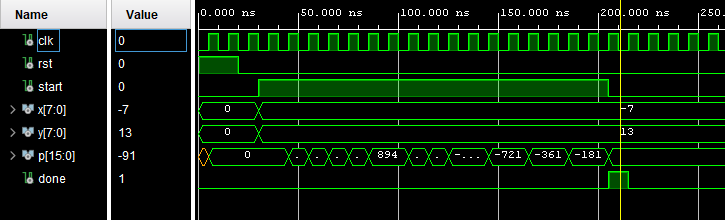
\includegraphics[width=0.95\linewidth]{figure/esercizio7-1/simulazione}
  \caption{Simulazione del moltiplicatore di Booth}
  \label{fig:esercizio7-1:simulazione}
\end{figure}

Il caso simulato è $(-7) \cdot 13$: \texttt{x} vale $-7_{10}$ (0xF9, $11111001_2$) e \texttt{y} vale $13_{10}$ (0x0D, $00001101_2$). Dopo il rilascio del reset, \texttt{start} passa a \texttt{'1'} e \texttt{p} attraversa i prodotti parziali durante gli otto passi (nella forma d'onda compaiono, tra gli altri, i valori $-721_{10}$, $-361_{10}$ e $-181_{10}$). A circa 200 ns \texttt{done} si porta a \texttt{'1'} e \texttt{p} vale $-91_{10}$, coincidente con il valore atteso.

\begin{risultato}
Con \texttt{x} $= -7$ e \texttt{y} $= 13$, all'attivazione di \texttt{done} l'uscita \texttt{p} vale $-91$, come previsto dall'\texttt{assert} del testbench.
\end{risultato}
